\section{KPIX Silicon Tracking}
Most recent update: 2020-05-1135 \\
Contact person: Marty Breidenbach (email: mib@slac.stanford.edu)
Contact person: Marcel Stanitzki (email: marcel.stanitzki@desy.de)
Contact person: Mengqing Wu (email: mengqing.wu@desy.de)
\subsection{Introduction}

The design of the SID Tracker is based on \cite{Behnke:2013lya},


\begin{figure}
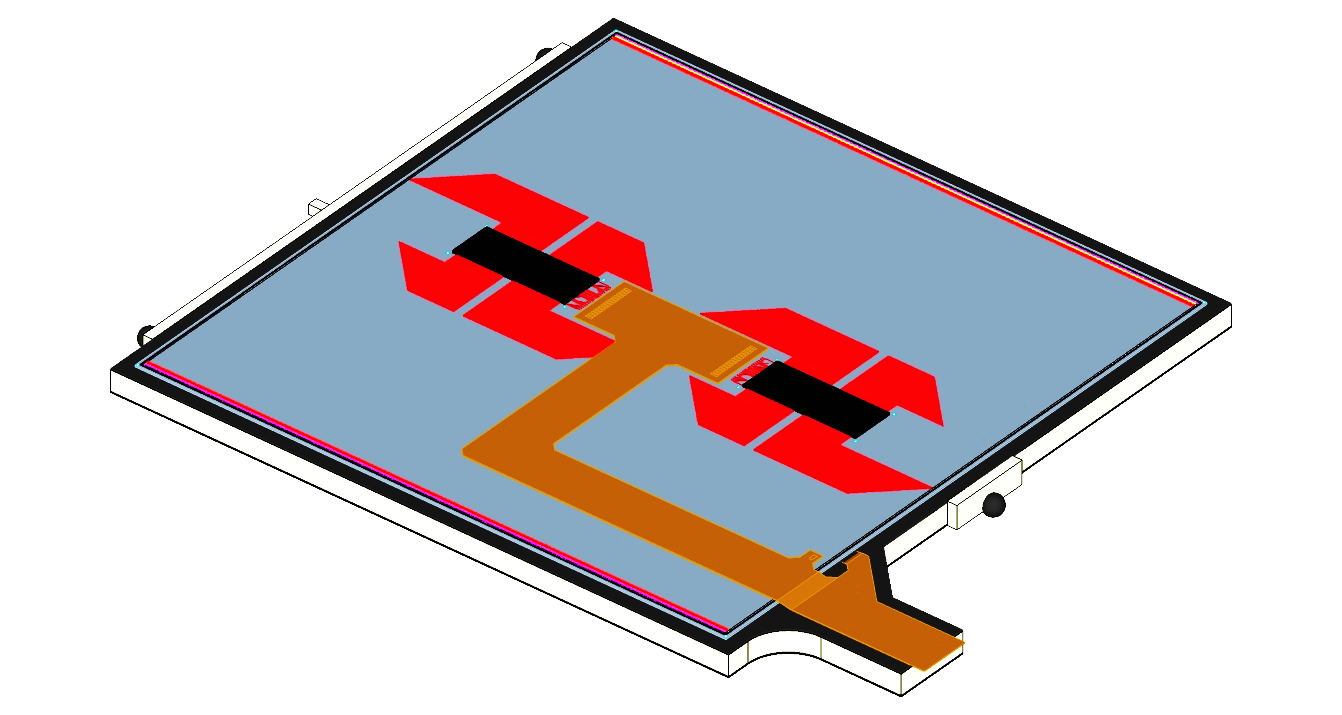
\includegraphics[width=0.49\textwidth]{Tracker/KPIX/Tracker_Module_SiD_Drawing.png}
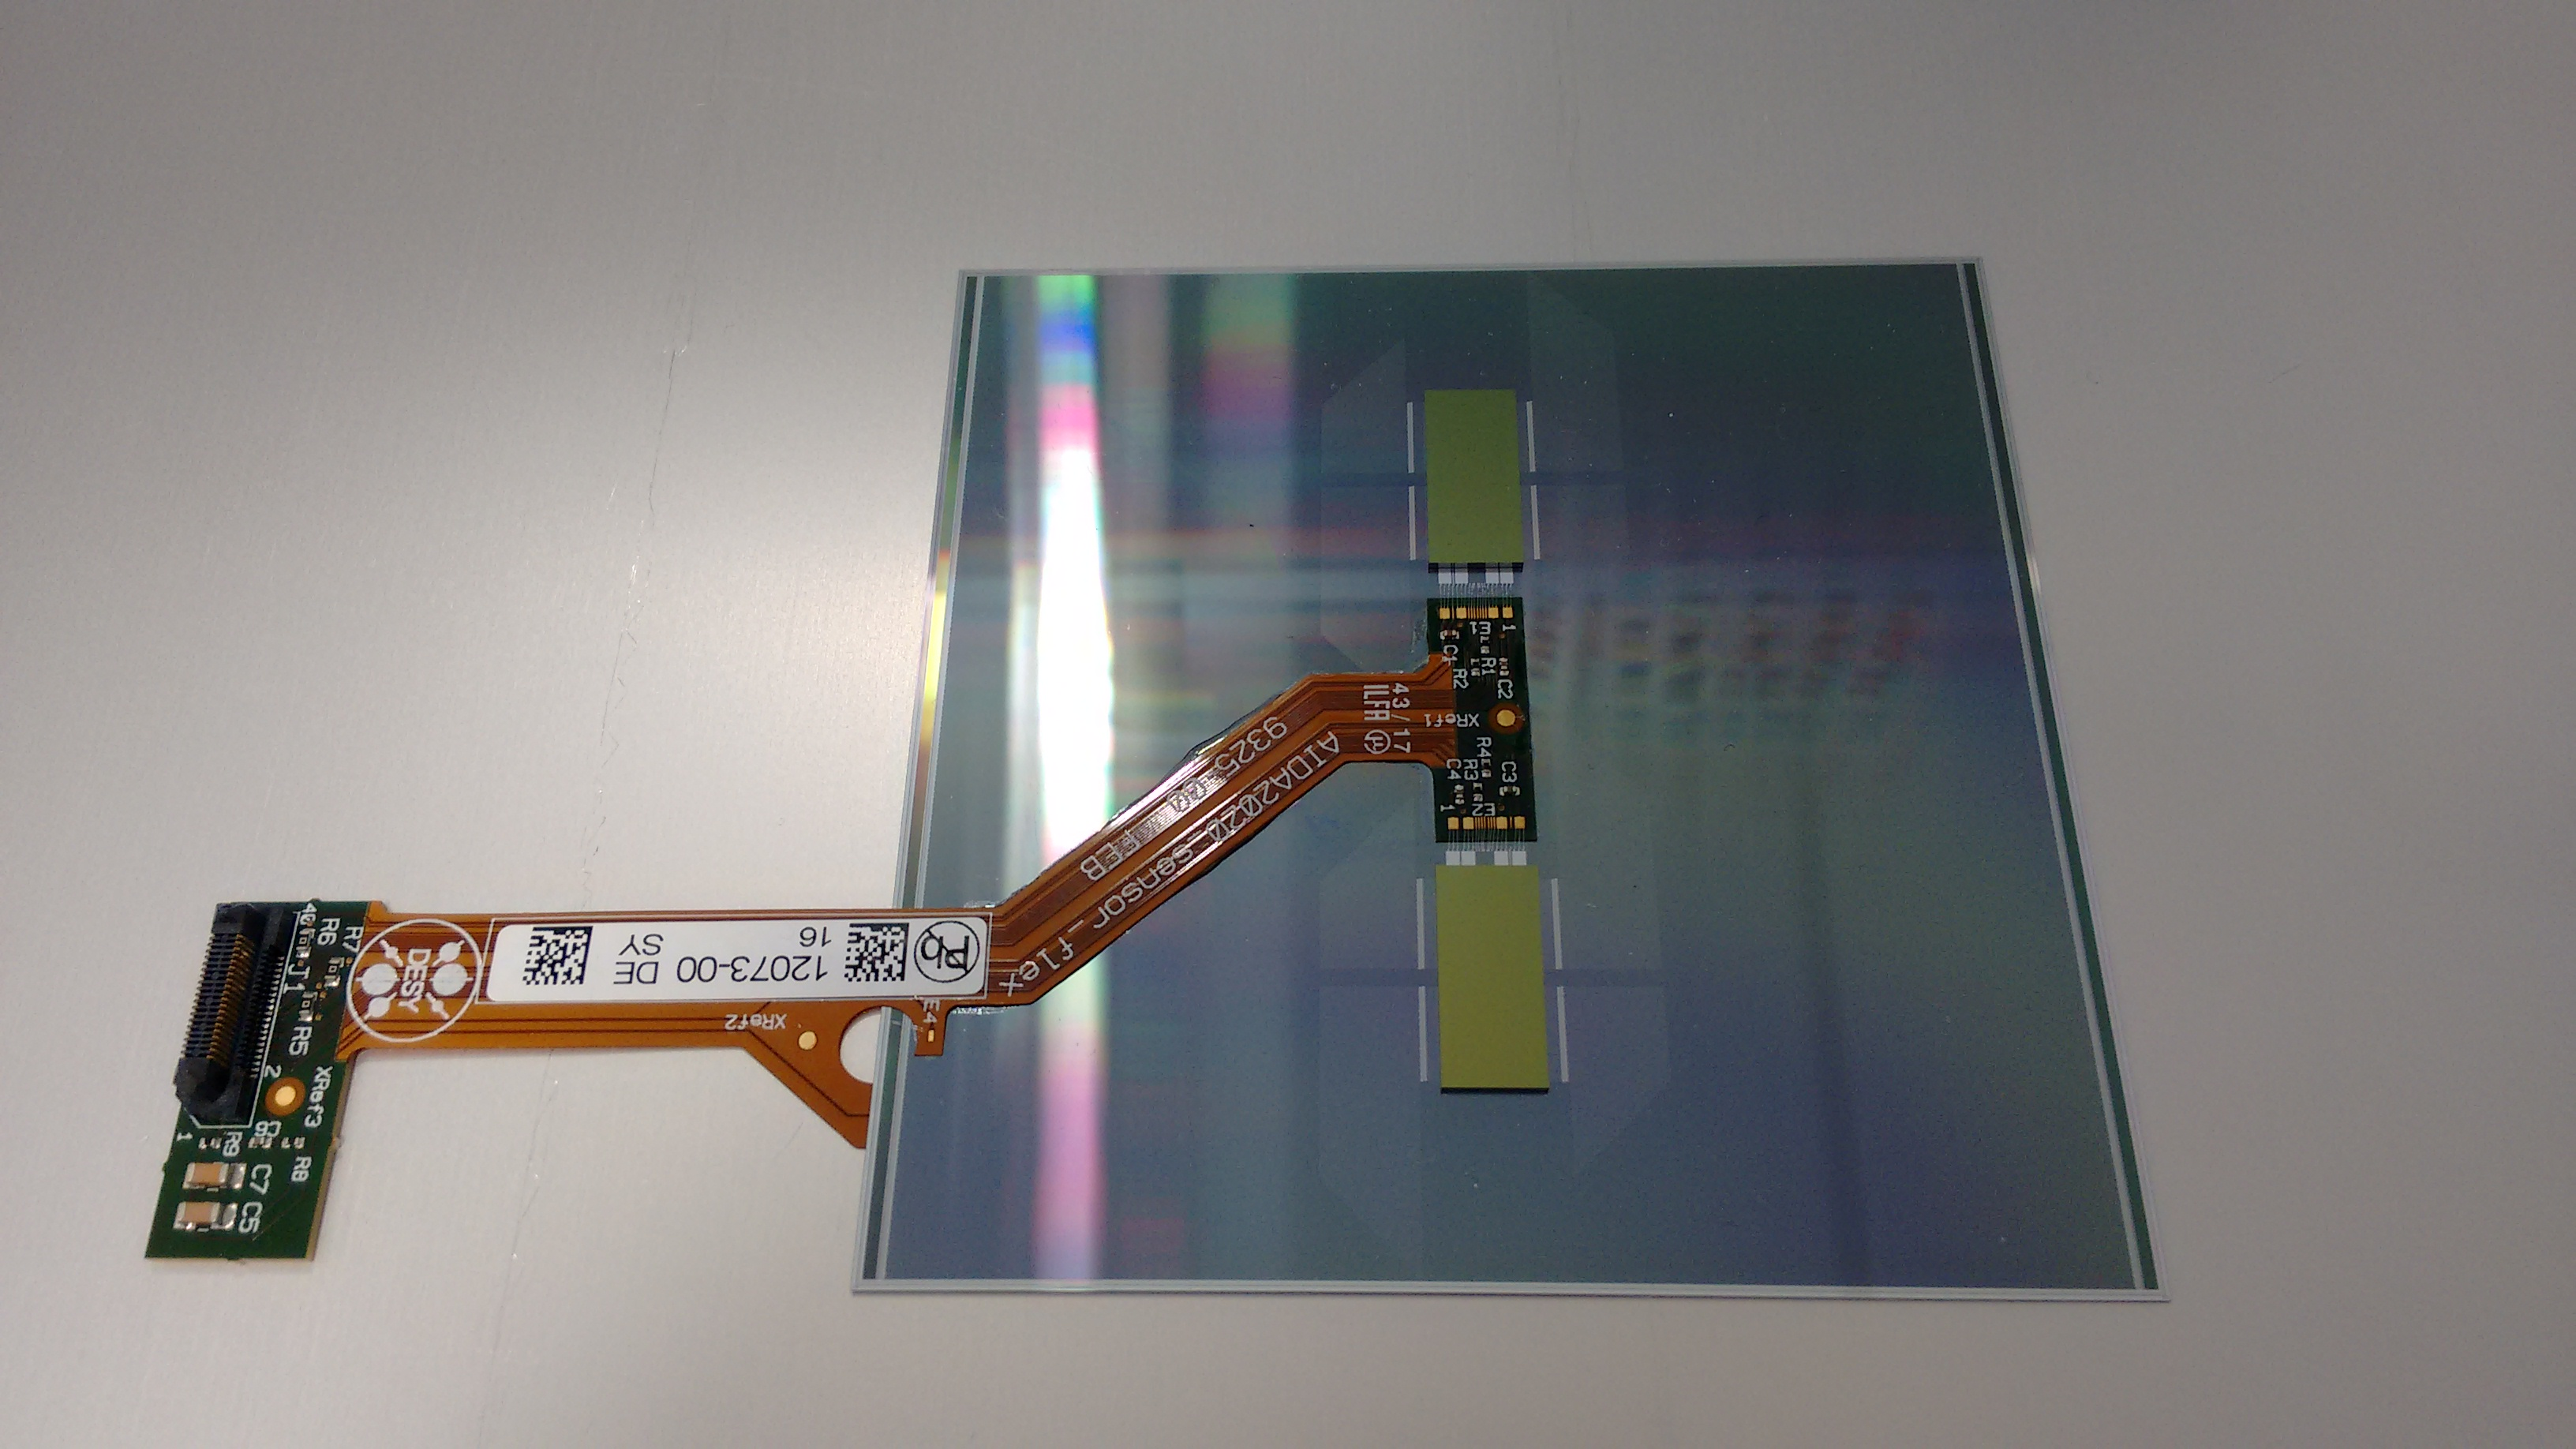
\includegraphics[width=0.49\textwidth]{Tracker/KPIX/Tracker_Module_SiD_Photo.jpg}
\caption{This SiD Tracker Module as foreseen for the baseline SiD Tracker\cite{Behnke:2013lya} and a first prototype sensor completely assembled}
\end{figure}


KPiX is a 1024 channel ``System on a Chip'' intended for bump bonding to large area Si sensors, enabling low multiple scattering Si strip tracking and high density Particle Flow calorimetry for SiD at the International Linear Collider (ILC). Each channel consists of a dynamically switchable gain charge amplifier; shaping; threshold discrimination; and 4 sample and hold capacitors and 4 timing registers. The chip permits 4 separate measurements of amplitude and time of threshold crossing during each train, and amplitude digitization and readout during the intertrain period. The dynamic range is from sub minimum ionizing particle (mip) (in \SI{320}{\micro\meter} silicon) to more than 2000 mip. KPiX also has a calibration system for each channel, servos for leakage compensation, ``DC'' reset for asynchronous operation for testing with cosmic rays, and polarity inversion for use with GEMs and similar detectors. The noise floor is about \SI{0.15}{fC} ($\simeq$ 1000 electrons), and the maximum signal is \SI{10}{pC} (utilizing the dynamic range switching). The full dynamic range corresponds to 17 bits.

\subsection{Recent Milestones}
ILC related R\&D in the US has been largely unfunded and small efforts are being kept alive. The KPiX R\&D is such an example of necessary work for SiD.

\item Tracker Sensors: The current prototypes will be evaluated, and if appropriate tested in a beam.

Future sensors will be ordered with Au pads.

An additional issue is that the Tracker sensor was planned to be wire bonded to its (very thin) cable. The sensor oxide layer is not strong enough to allow wire bonding without damage, and so must be solder bumped. The pad pitch is small, and solder bumping the cable will be challenging. The trouble with the wire bonding to the sensor was unexpected.

\subsection{Engineering Challenges}
At this time, KPiX is seen as the baseline readout system for the tracker and electromagnetic calorimeter. A stack of 13 EMCal sensors with bump bonded KPiX was assembled for a beam test at SLAC in the summer of 2013. That test discovered that two kinds of crosstalk are significant:
\begin{itemize}
	\item In-time crosstalk occurs due to parasitic coupling of traces on metal 2 of the sensor to other pixels. The level of crosstalk increases with the size of the signal, and decreases with increased speed of the front end charge amplifier (meaning increased current and power dissipation).  A new sensor design is being developed that uses metal 1 to shield the traces of metal 2, and these ideas will be tested in the next sensor prototype.
	\item Out-of-time cross talk occurs when many pixels are hit and reset simultaneously. The resets collectively cause other pixels to trigger, and a cascade builds up. This uses up all the KPiX buffers. The root cause of the problem appears to be some internal logic within KPiX that is not current limited, and will require design modification.
\end{itemize}


Another concern is that the current design of KPiX has deadtime after a pixel has accepted a trigger. Only the triggered pixel is affected; all the other pixels are available for signals. This deadtime is different from the usual notion of data acquisition deadtime where the entire detector is unavailable, but the correction to the luminosity integral is easy. Finally, the buffer requirement (4 in the current version of KPiX) is being re-evaluated in SiD simulations. A possible new architecture for KPiX is in early stages of evaluation.
A small mechanical engineering effort has started to study the structure of the EMCal. The Sid EMCal has emphasized thin gaps between the tungsten layers to minimize the Moliere radius, and this implies that the structure is connected by columns at the vertices of the sensors. The DBD design shows hexagonal sensors, which indeed are the most efficient way of tiling large areas, but no consideration was given to the edges of these arrays. The design is being re-evalutated to optimize the cost-effectiveness over the whole area taking into account geometric efficiencies and total wafer cost.
Tracker sensors are now at IZM for the pad plating and subsequent bonding of KPiX; they will then go to UCD for cable attachment and testing.


\subsection{Future Plans}
Assuming positive developments with Japan are announced soon, we expect the financial support to improve. It should be noted that an important effect of the withdrawal of support is that most of the US collaborators have been forced to move to other work.
\begin{itemize}


	\item KPiX: A new architecture with little (or no) deadtime will be evaluated. A decision will be made to develop this new architecture or incrementally.
	\item improve the existing design.
\subsection{References}

\end{itemize}
